\section{Literature Review}

\subsection{Theories of Motivation}

There are many theories of how people learn, how to teach, and how to engage with students. 
In this proposal, I investigate Academic Motivation - the process by which people choose to direct energy towards learning.
Motivation is well understood to be a crucial part of education, particularly in Computer Science~\cite{Carter:2011}.

\subsubsection{MUSIC Model of Academic Motivation}

My work uses the MUSIC Model of Academic Motivation as its primary motivational framework.
The decision to use the MUSIC model was based on several criteria.
Although there are many motivational models available, few strive to be holistic models specifically developed for academics.
For example, theories like Expectancy-Value and Cognitive Evaluation Theory have a wider scope and have stemmed from other disciplines such as healthcare. %TODO: Cite
The MUSIC Model is derived from a meta-analysis of these other theories, incorporating only the academically relevant components.
Further, the MUSIC model is a tool meant for both design and evaluation, allowing it to be used in all phases of this work.
Finally, the model and its associated instrument, the MUSIC Model of Academic Motivation Inventory (MMAMI) , has been extensively validated and used in other educational domains, making it a reliable device\cite{jones-validity}.

The MUSIC model identifies five key constructs in motivating students \cite{jones-description}.
\begin{description}
	\item[eMpowerment:] The amount of control that a student feels that they have over their learning (e.g., course assignments, lecture topics, etc.). This is amount of Agency that a student perceives.
	\item[Usefulness:] The expectation of the student that the material they are learning will be valuable to their short- and long- term goals. There is no clear delineation of the time-scale for these goals, but there is nonetheless a distinction between strategic skills that students need to be successful in careers and personal interests and the tactical skills they need to complete present-day tasks.
	\item[Success:] The student's belief in their own ability to complete assignments, projects, and other elements of a course with the investment of a reasonable, fulfilling amount of work. Most students desire experiences that are successful, but still challenging enough to be worth it.
	\item[Interest:] The student's perception of how the assignment appeals to situational or long-term, individual interests. The former covers the aspects of a course related to attention, while the latter covers topics related to the fully-identified areas of focuses of the student. It can be difficult to parse out the difference between individual interests and long-term career goals -- there can be alignment between these two components.
	\item[Caring:] The students perception of other stakeholders' attitudes toward them. These stakeholders primarily include their instructor and classmates, but also can be extended to consider other members of their learning experience (e.g., administration, external experts, etc.). It can also be viewed as the extension towards society as a whole.
\end{description}

Students are motivated when one or more of these constructs is sufficiently activated.
They are not all required to achieve maximal levels, and in fact that is not always desired -- it is possible, for instance, for a student to feel too empowered, and become overwhelmed by possibilities.
For some of these constructs, a careful balance is required, and it may not be possible to ever achieve a minimal level; no matter how exciting you make your lecture, you may never convince your students it is interesting, although it is possible that they will still consider it useful and stay motivated.
Crucially, students' subjective \textit{perception} of these constructs is a defining requirement and is more important than objective reality.
It does not matter if you believe that your lecture is Useful, if you have not convinced your students that it is (although an instructor's beliefs are a powerful tool for convincing their students).

The MUSIC model is often used as an organizational framework and an evaluative tool.
As the former, it is a list of factors to consider when building modules, assignments, and content of a course.
At all times, instructors can consider whether they are leveraging at least one construct to motivate their students.
As the latter, it offers both a quantified instrument (MMAMI) and a structure to anchor a qualitative investigation on.
The model has also been used in course design: Jones describes a controlled classroom experiment to motivate students by having an experimental group reflect on how a course satisfies the constructs of the MUSIC model. Students were simply prompted to answer the question ``How will the material presented here be useful to you?''.
Quantitative data gathered after the experiment indicated a significant increase in motivation~\cite{mcginley2014brief}.
The MUSIC model is therefore a flexible resource for studying motivation.

The MUSIC model has not been applied to Computer Science education before, although a number of other motivational frameworks have been leveraged in studies.
Many of these studies often find results that hint at many of the elements of the MUSIC model.
For instance, Mitchell describes interest, usefulness, and ``intellectual challenges'' (success) as three primary elements influencing success in computer science~\cite{Mitchell:2000} .
Although they do not discuss empowerment and social elements, many other studies often suggest these themes.
Still, it should be acknowledged that it is an open question whether the MUSIC model can be applied directly, or if the domain has different characteristics from other disciplines.

\subsubsection{Situated Learning Theory and Authenticity}

Although most of this proposal relies on the MUSIC Model of Academic Motivation due to its holistic explanation of motivation, it is also useful to explain elements of my research in terms of Situated Learning Theory in order to explain aspects more directly connected to students' learning (as opposed to just motivation).
Situated Learning Theory, originally proposed by Lave and Wenger, argues that learning normally occurs as a function of the activity, context, and culture in which it is situated~\cite{lave-situated}.
Therefore, tasks in the learning environment should parallel real-world tasks, in order to maximize the \textit{authenticity}.
Contextualization is key in these settings, as opposed to decontextualized (or ``inert'') settings.
The key difference is that learning is driven by the problem being solved, rather than the tools available. Therefore, the problem being solved should lead directly to the tool being taught.
This argument suggests that this is a key aspect of motivating students.

Authenticity is a crucial, recurring theme within Situated Learning Theory.
All instruction and assessment must be aligned with reality such that success in the former leads to success in the latter.
However, there is a subtle nuance here -- authenticity is a perceived trait, not an objective one.
Students derive value from their learning only if they \textit{perceive} authenticity, regardless of whether the instructor has successfully authenticated the experience.

Situated Learning Theory has been applied to Computer Science before, with mixed results. A seminal paper by Ben-Ari \cite{ben2004situated} explores its application and limitations.
This paper is somewhat hasty in its application of SL Theory by taking a macro-level view -- they narrowly look to Open-Source and Industry Software Development communities as the only potential Community of Practice and interpret SL Theory as strictly requiring constant legitimacy, largely ignoring the possibility for gradual development of authenticity within individual courses and modules throughout a curriculum:

\begin{quote}
What I am claiming is that situated learning as presented in their work cannot be accepted at face value, because it simply ignores the enormous gap between the world of education and the world of high-tech CoPs, which demand extensive knowledge of both CS subjects and applications areas.
This gap can only be bridged by classical decontextualized teaching in high schools, colleges and universities.
\end{quote}

However, other researchers have found it a useful lens for analyzing curricula.
For instance, Guzdial and Tew \cite{guzdial2006imagineering} used the theory to explore and deal with the problem of inauthenticity within their Media Computation project.
SL Theory clearly has value, but only as a function of the way that it is applied.
In this preliminary proposal, I use SL Theory as a generalized tool for exploring the topic of authenticity throughout introductory Computer Science.

The original work in Situated Learning Theory was not about pedagogy or instructional design. It described how people learn and the importance of context and collaboration, but it did not recommend a particular teaching style.
Subsequent research by Brown \cite{brown1989situated} and others expanded the theory so that it could be applied to the design of learning experiences.
These expansions often naturally dictate the use of active learning techniques, reducing the role of lecture in favor of collaborative, problem-based learning activities.
Choi \& Hannafin \cite{situated-cognition} describe a particularly useful, concrete framework for designing situated learning environments and experiences.
The Choi \& Hannafin framework has four key principles: the Context, described as the ``... The problem's physical and conceptual structure as well as the purpose of activity and the social milieu in which it is embedded''\cite{rogoff1984everyday}; the Content, the information intending to be conveyed to the students; Facilitations, the modifications to the learning experience that support and accelerate learning (commonly done through Scaffolds); and Assessment, the methods used to evaluate the learning experience and measure the progress of the student.
	
\subsubsection{Contexts vs. Content}

\begin{wrapfigure}{R}{0.5\textwidth}
		\begin{center}
				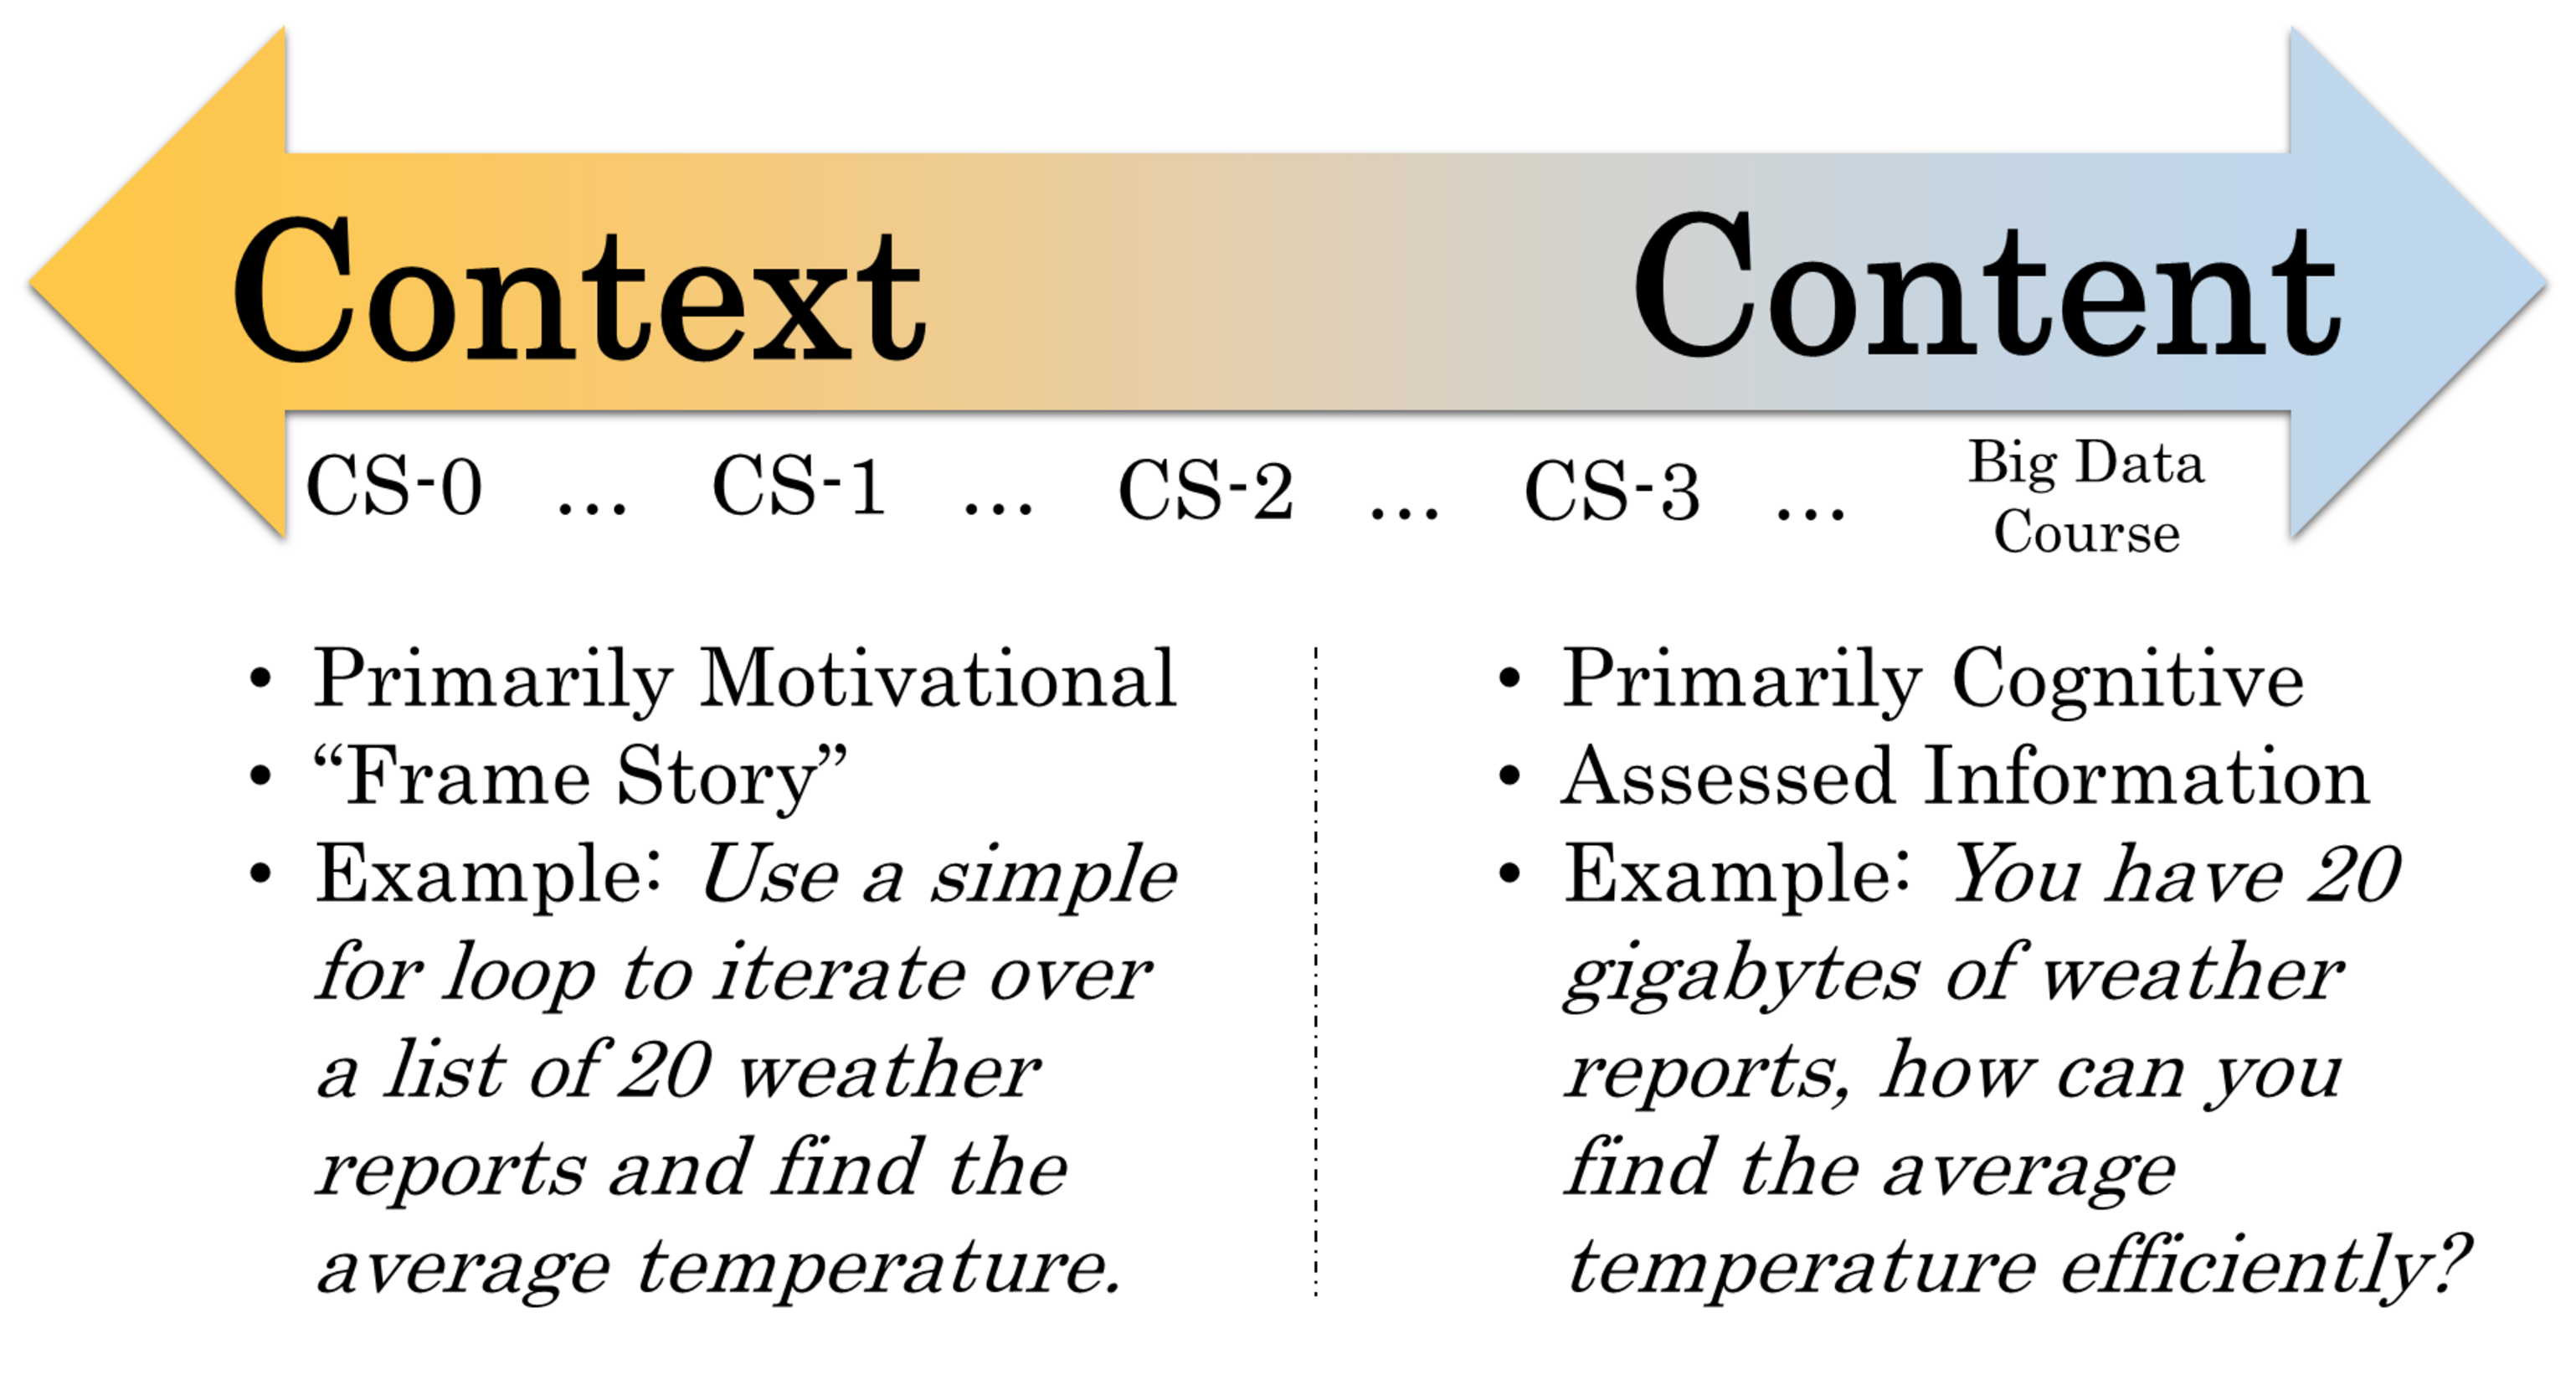
\psfig{file=images/content-context-2.eps, width=\linewidth}
		\end{center}
		\caption{Content vs. Context}
		\label{fig-content-context}
\end{wrapfigure}

There is a reciprocal relationship between contexts and content.
Figure \ref{fig-content-context} demonstrates an example of this relationship for the expected emphasis on big data as a context vs. content throughout an undergraduate curriculum, from a CS-0 (non-majors) course all the way to an upper-level course specifically on big data.
Just as the upper-level course would naturally use big data as its context and content, a CS-0 course could still have content related to big data.
However, the majority of the use of big data would be as the framing story for assignments, especially in earlier parts of the course.
When students learn programming in the context of, say, game development, they are almost necessarily learning content related to game development that may not be universal to computer science (e.g., how graphical resources are organized and accessed within the game engine).
This content may be seen as a distraction by the instructor, or as useful side knowledge. For example, if a student had to learn how to use a command line in order to compile their game, they would be learning an authentic skill that might not be considered part of the core content, but is nonetheless generally useful.
When evaluating a context, it is useful to consider what content it represents, and how authentic and useful it is.
The authenticity of content that is attached to a context affects the authenticity of the learning environment as a whole.
A good context enables a student to find recognizable elements and build on prior understanding, eventually being able to freely transfer their learning to new contexts.

Fascinatingly, the need for a strong context diminishes as learners mature and become domain-identified -- the content itself becomes the context.
Learners start to see other contexts as nothing more than distractions and unnecessary fluff.
This makes sense -- you would hope that Computer Science majors in their third semester would be naturally interested in the material, and this is borne out in experimental data.
For instance, Yarosh \& Guzdial attempted to integrate Media Computation in a CS-2 (Data Structures) course, and found that the learners had ``outgrown the desire for a context''~\cite{yarosh2008narrating}. 
These results are similar to results we found in our interventions with a CS-3 couse on Data Structures and Algorithms, where students seemed more irked by the surrounding context than intrigued.


\begin{figure}[!ht]
	\begin{center}
		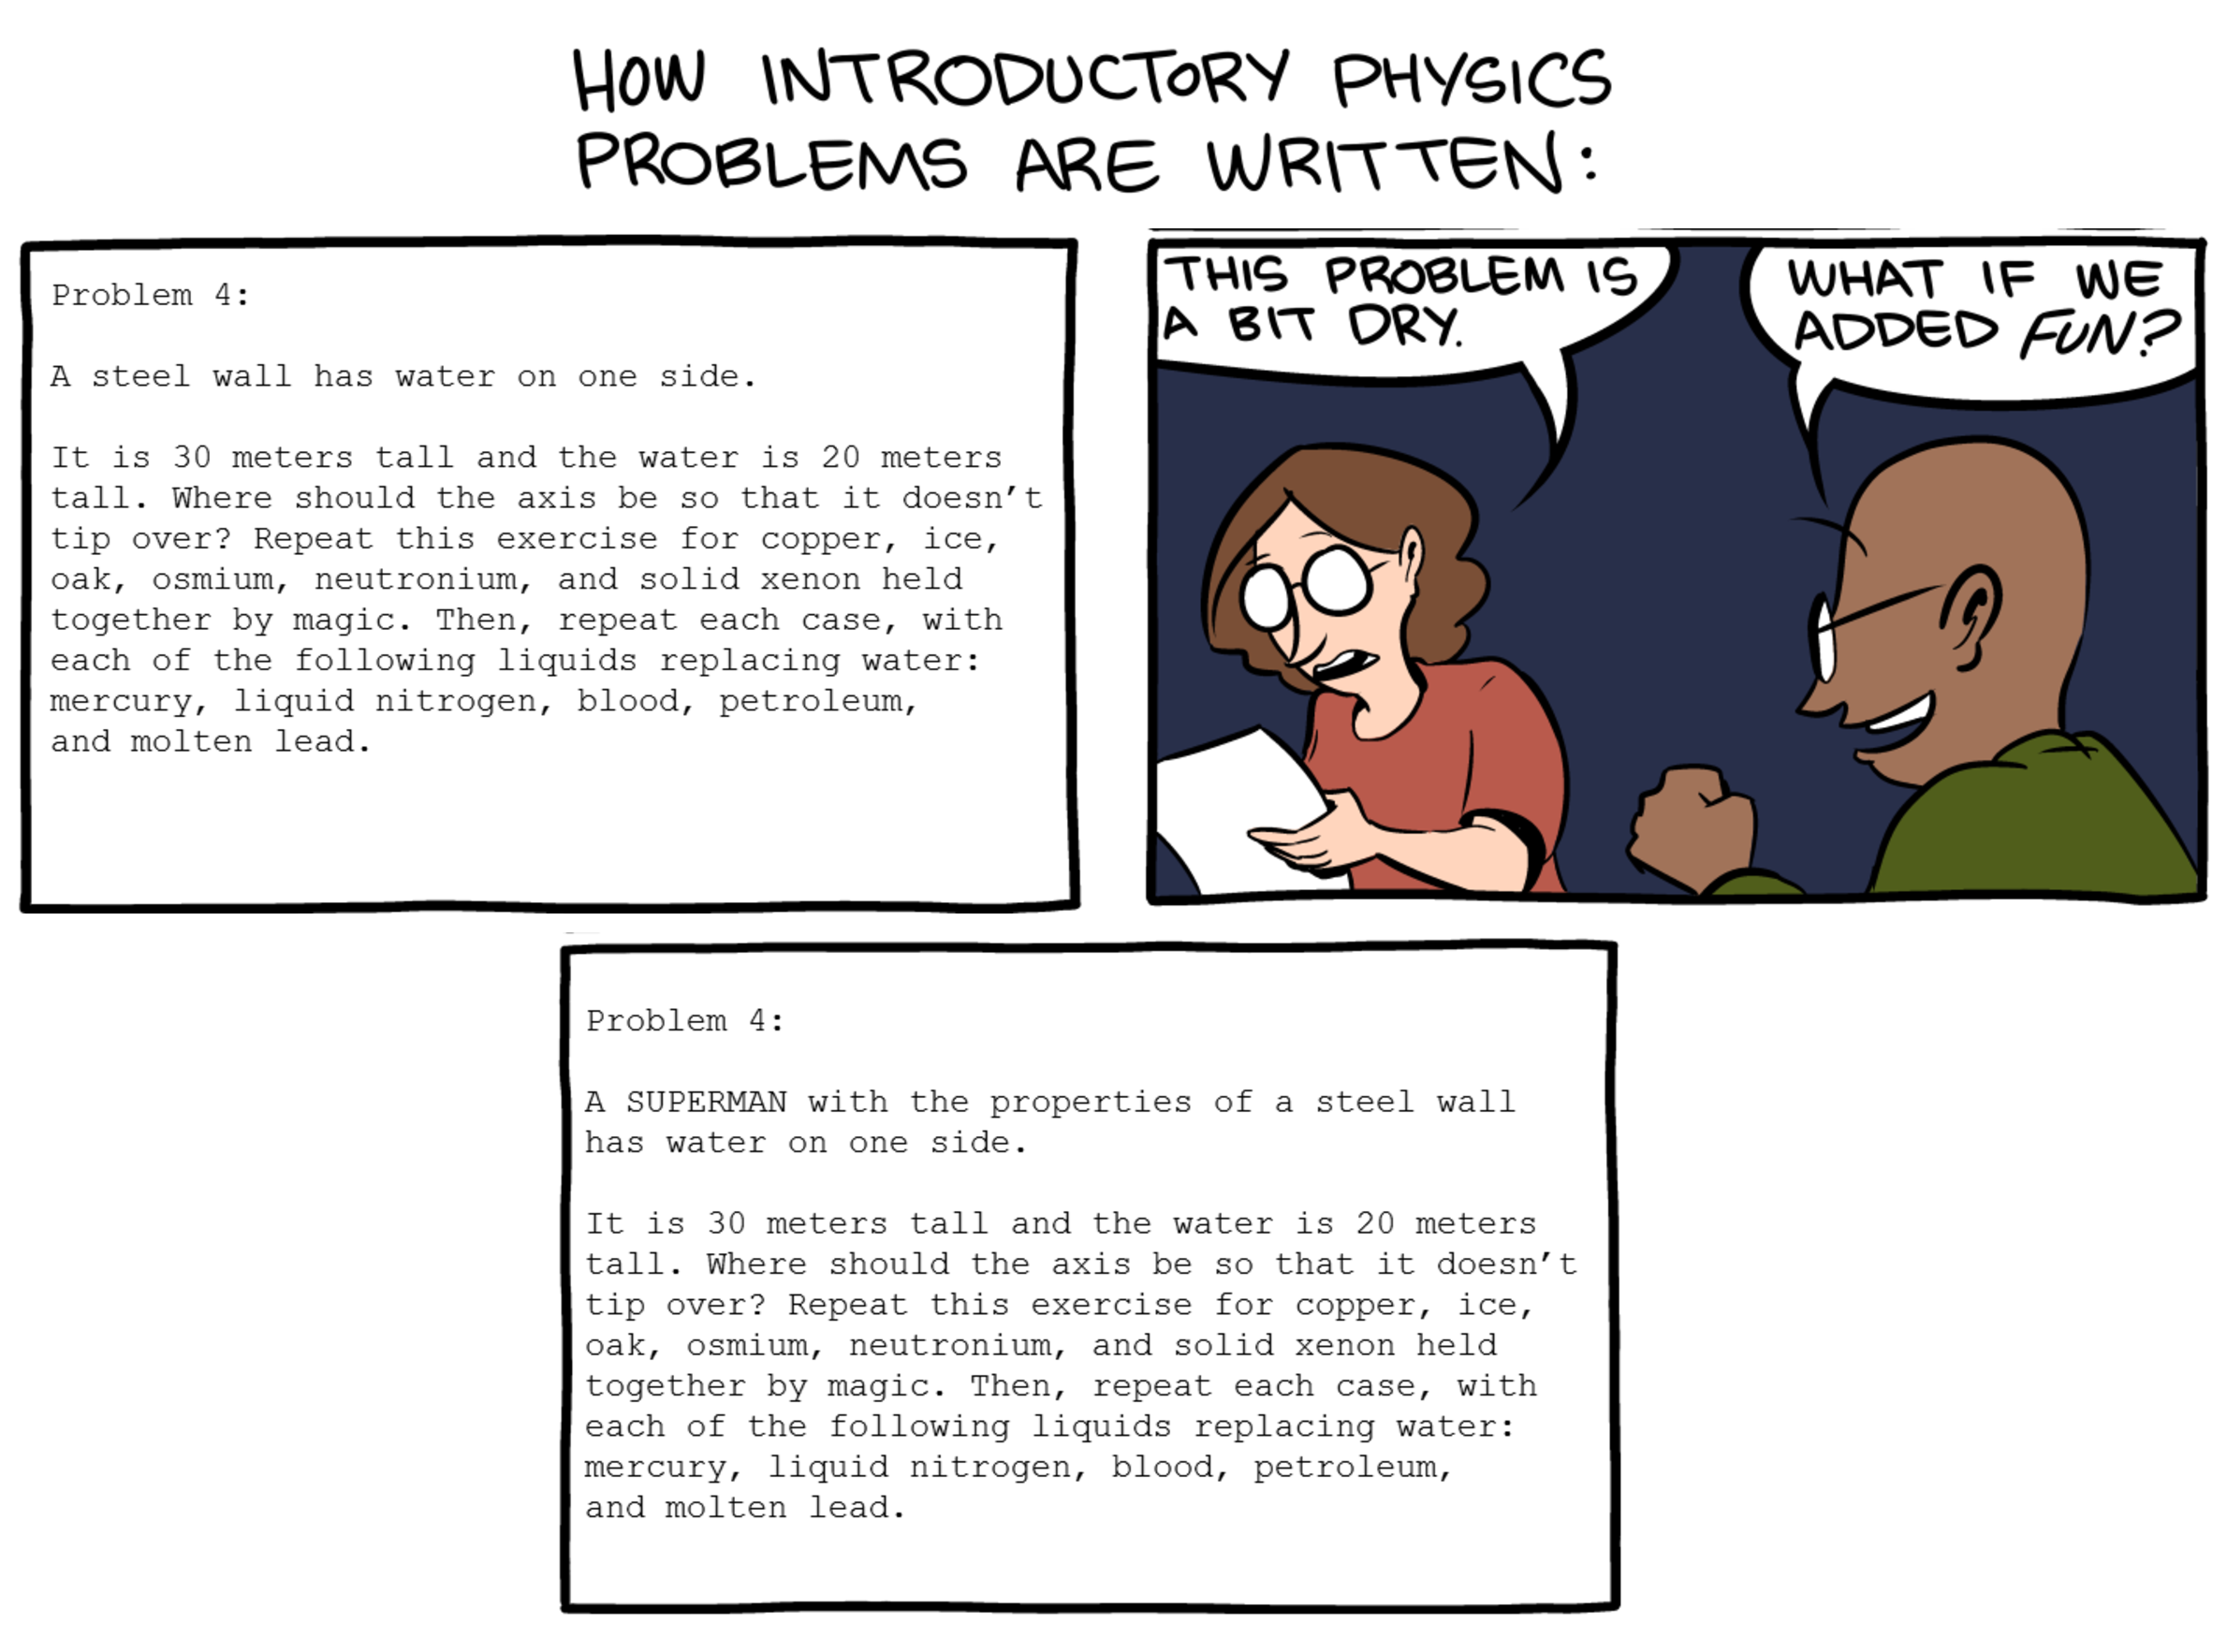
\psfig{file=images/smbc.eps, width=\linewidth}
	\end{center}
	\caption{How to Add Fun to Education}
	\textit{Making the context ``Fun'' is not necessarily trivial, whether in physics education or computer science education.~\cite{SMBC}}
	\label{fig-comic-context}
\end{figure}

Of course, it is up to the instructor to determine the depth and breadth of the context's integration.
The trade-off between the value and distraction added by the context is a delicate formula.
Consider the scenario in Figure \ref{fig-comic-context}.
A steel wall is a relatively relatable concept for most students -- they can readily imagine such a large, durable object, and it somewhat reasonable to expect that objects would interfere with it.
In this scenario, the instructors consider replacing the wall with a comic book character -- something that they anticipate will be more ``fun''.
If they are in tune with their learners, this might be an effective context -- perhaps they know that their learners are comic book fans.
However, because the integration is only at the surface level, it is possible that the learners will see this as a forced reference, and they will have a more negative reaction.
It is also possible that they will not recognize the reference, or feel no positive emotions with it -- many contexts do not take into account gender, racial, or socio-economic characteristics of the anticipated learner.
I suggest that the process of motivating students using a context is non-trivial, and in the following section I will explore prior work in contexts for Computer Science Education.

\subsection{Introductory Computing Content}

Different Computer Science programs have different introductory curriculums, varying on whether they focus on Object-Oriented programming, Functional programming, etc. 
Complicating this discussion is the bifurcation of undergraduate introductory computing into Computational Thinking (sometimes referred to as CS-0) and Computer Science (sometimes referred to as CS-1), and the simplified curriculums used in K-12 education (e.g., the new AP CS course).
However, It is commonly that any good introductory computing course will cover abstraction (representing complex phenomena more simply, usually as coded data), some form of decision-making (e.g., \texttt{if} statements, \texttt{cond} statements), and some form of iteration (e.g., \texttt{for} loops, recursion)~\cite{Kramer:2007, CS2013, csta-computational-thinking}.
From there, different curriculums lay out the material differently.
The ``How to Design Programs'' curriculum emphasizes a functional programming model, using a LISP-descended language named Racket, and the only looping mechanism that students are taught is recursion.
The dominance of the Object-Oriented Model in software engineering usually leads to a strong emphasis in introductory courses on abstracting data using Objects and Classes -- such as the ``Objects First'' curriculum.
Besides the technical aspects, definitions include softer skills such as a tolerance for unstructured problems and collaborative attitudes~\cite{csta-computational-thinking, google-computational-thinking}.

This proposal does not take a view on what should be included in an introductory experience, beyond a core of Abstraction and Algorithms.
However, for practical purposes, materials and research work are grounded and tested in some course, and have adaptions for that content.
Specifically, the proposed work is used in a Computational Thinking course, so that is how the content is oriented.
``Computational Thinking'' was coined by Seymour Papert in 1993~\cite{papert1996} and popularized by Dr. Jeannette Wing's 2006 paper~\cite{wing2006}, which opened a floodgate of discussion about the term. 
Unfortunately, there is still limited consensus on \textit{what} exactly CT is, whether it should be universally taught, how it should be taught, and how to identify when it has been taught.

An excellent resource for summarizing the history of Computational Thinking research is the 2013 dissertation by Wienberg~\cite{weinberg2013}. 
This comprehensive survey analyzed 6906 papers directly or indirectly related to Computational Thinking from 2006-2011, describing research efforts and findings.     
Over half of the research on CT describes approaches to pedagogy (Curriculum and Program Description), leaving a small amount to modeling (Philosophy and Opinion) and assessment (Research and Evaluation). 
The lack of assessment research is understandable given the youth of this area of research, but still troubling.
Even more troubling, however, is the further analysis of the 57 empirical studies.
Only fifteen (26\%) studies include or sought an operational definition of computational thinking, and only six go beyond the superficial (solely describing computational thinking as a ``way of thinking'', a ``fundamental skill'', or a ``way of solving problems''). 
The failure to identify an operational definition weakens the theoretical strength of the studies.
This weakness likely stems from the background of the researchers: only 18\% of the articles involved education experts.
In other words, over four-fifths of this educationally-oriented research appears to have been performed by people with no real formal training in educational research techniques.
This is particularly troubling given that Computational Thinking is a strong target for interdisciplinary endevaors.

Weinberg reflects on the continuing debate about the importance of Computational Thinking:
\begin{quote}
    Many, like Wing, believe computational thinking to be a revolutionary concept, one as 
important to a solid educational foundation as are reading, writing, and arithmetic (Bundy, 2007\cite{bundy2007}) 
(Day, 2011\cite{day2011}). Others believe its potential and significance are overstated (Denning, 2009\cite{denning2009}; 
Hemmendinger, 2010\cite{hemmendinger2010}), and some have voiced concern that by joining forces with other 
disciplines computer science might be diluting either one or both of the participating disciplines 
(Cassel, 2011\cite{cassel2011}; Jacobs, 2009\cite{jacobs2009}). Both the praise and the criticism for computational thinking could 
perhaps be tempered by reflecting on a historical quote by Pfeiffer in 1962: “Computers are too 
important to overrate or underrate. There is no real point in sensationalizing or exaggerating 
activities which are striking enough without embellishment. There is no point in belittling 
either.” (Pfeiffer, 1962\cite{pfeiffer1962}).
\end{quote}

Although it is ambiguous what Computational Thinking is, we will take it as a given that it requires students to learn some amount of non-trivial programming: using iteration constructs (e.g., \texttt{while}, \texttt{for each}, recursion, etc.), decision constructs (e.g,. \texttt{if}, \texttt{unless}), have some sense of program state (through mutating variables or passed through composed functions), and require the programmer to translate instructions into a form the computer can understand.
This is not meant to be a strict definition of everything a programmer should learn -- simply an acceptable, minimal subset.

\subsection{Introductory Computing Contexts}

As part of the overarching goal to bring more students into Computer Science, a large number of contexts have been explored in Introductory computing. 
The context of a learning experience grounds the learner in what they already known, in order to teach the new material.
Many introductory computing experiences focused on presenting the content as purely as possible, which can come across as abstract and detached~\cite{Zografski}.
However, starting with Seymour Papert's work with robotics and the LOGO programming environment in the 70s~\cite{papert1996}, instructors have been interested in motivating students' first experience with richer contexts.
Some of these contexts rely on Situational Interest (e.g.,  Digital Media ``Computation'' (Manipulation)~\cite{Forte} and Game Design~\cite{Zografski}), while others attempt to provide enduring career value (e.g., [Big] Data Science ~\cite{Anderson}) or short-term social applicability (e.g,. Problem Solving for Social Good~\cite{SocialGoodinComputingEducation}).
Ultimately, each of these approaches draws on different facets of motivation, they may be compatible with each other.
In this section, I will discuss the implications of these different approaches.


\subsubsection{Abstract Contexts}

Denning describes the early perception of Computer Science by the public as ``stodgy and nerdy''~\cite{Denning:2005}, since many early computer science classes were driven so strongly by mathematics and logic.
A common early introductory programming problem, for instance, is writing a function to compute a Fibonacci number -- a relatively simple task if you are familiar with the recurrence, and one that leads quite nicely to discussions on the implementation of algorithms, computational complexity, and a host of other subjects~\cite{crazypantsfibonaccipaper}.
These contexts are ``abstract'' because they are already at a similar level of abstraction as the content they are attempting to convey.
However, Oliveira~\cite{ConcreteVsAbstract} suggests that the discussion about ``abstract vs. concrete'' contexts is a misleading one, because the purity with relation to the content is less important than \textit{prior knowledge}.
According to modern constructivist and cognitivist theories, learners build on prior knowledge, and the ability to relate to what they know is crucial.
The simple fact is that most students are not particularly good at mathematics, so relying on it as a context is not a useful approach compared to finding subjects that students know and understand readily.

\subsubsection{Situationally Interesting Contexts}

As it became clear that Computer Science had a serious image problem, work began on making Computer Science ``fun'' and approachable. 
A key goal was to increase diversity and to broaden participation. 
This led to the rise of Situationally Interesting Contexts, emphasizing problems and projects that would be immediately appealing to a wide audience.
Guzdial, for instance, was largely responsible for the creation of the Media Computation approach, where students use computational techniques (e.g., iteration and decision) to manipulate sound, images, videos, and other digital artifacts.
As an example, students might use a nested, numerically-indexed \texttt{for} loop in order to adjust the red-value of the pixels in an image, treating it as a two-dimensional array of binary tuples, in order to reduce the red-eye of a photo.

Although wildly deployed, a review of these curricular materials by Guzdial \cite{guzdial2006imagineering} in light of Situated Learning Theory found that students did not find this an authentic context, and intense rhetoric was insufficient to convince them that it was authentic. 
Few students find it expedient and helpful to remove the red-eye from family photos by writing python scripts, and so are unconvinced that the context has long-term value to them (regardless of whether the content does).
Guzdial leaves open the question of what contexts can be truly authentic for non-majors, given the relative novelty of teaching introductory computing for non-majors.
Ben-Ari echos this question by suggesting a very narrow selection of authentic contexts and communities in his paper exploring the application of Situated Learning Theory to Computer Science in general \cite{ben2004situated}.
Critically, the opposite problem could occur -- if an instructor is effective at convincing students that a context is authentic, the students may believe the instructor even if the context is not authentic.
There are serious ethical issues involved in mispresenting the utility of a context, leading students to develop an embarrassing misconception of the field. Imagine a young child believing that all of Computer Science is game design, because that is what they started off doing.

There are other disadvantages of an Interest-driven approach.
The motivation literature describes ``Seductive Details'' (interesting but irrelevant adjuncts)~\cite{harp1998seductive} as interfering both with short-term problem completion and long-term transfer.
In other words, students get hung up on unimportant aspects of the context, so that they ignore the content.
Consider a student using the game and animation development environment Scratch, which allows beginners to create sprites from images.
A young learner might be so amused by the ability to change the color and shape of their image, that they neglect their assigned work.
Although a well-regulated learner would not be distracted, most of the at-risk population that would benefit from these contexts are unable to deal with such distractions.
Of course, this could be said of any context, but there is particular danger from a seductive context.

Kay~\cite{Kay:2011} identifies another, potentially critical problem of relying solely on situationally interesting contexts, particularly when it leads to individualized interest towards that context and not the content. 
What happens once a student has completed the introductory course and is ready to move onto further courses?
Most later courses are more decontextualized, and will not use contexts such as game development, robots, etc.
Kay goes so far to say that it is unethical to suggest to students that a contextualized introductory course is representative of the curriculum as a whole.

\subsubsection{Empowered Contexts}

Orthogonal to the idea of making a context fun is the idea of giving students more freedom and agency to control their learning.
Compared to Interest-driven contexts, this approach is comparatively less researched, although it is not an uncommon practice. Instructors will often allow students to choose from a range of projects or assignments.
Stone~\cite{EmpowermentInProjects} ran a 2-year study where students were allowed to choose their projects from a wide range of domain areas (e.g., Biology, Math, Business, Etymology), and were then surveyed on their engagement.
Unfortunately, their experiment suffered strongly from low enrollments and even lower survey responses. Therefore, it is difficult to believe any of their results (including the idea that women are more likely to prefer biological- and meterological-themed projects).
However, their experiences do suggest an interesting challenge: normalizing the difficulty (both in terms of computational knowledge and domain knowledge) across many different projects is a struggle.

\subsubsection{Contexts that Make Instructors Care}

Most modern educational theories argue that learning is inescapably affected by social factors.
There is evidence that the instructor~\cite{thompson2009engine} and fellow students~\cite{Barker:2009} are the most important factors in an introductory experience, for instance.
Kay~\cite{Kay:2011} discusses this explicitly.
It is possible that the most important element in a context is not whether it is fun or useful, but whether the instructor can get excited about it and impart that enthusiasm to the student.
And not just enthusiasm, but a thorough understanding of the problem, its usefulness, and the rest of its attributes.

\subsubsection{Useful-Driven Contexts}

An alternative focus to Interest is Usefulness, the idea that the context should have immediate or eventual benefit to the learner's needs.
To some extent, it is impossible (or at least prohibitively difficult) to find a one-size-fits-all context that will be useful to all learners (designing learning experiences without your learners in mind is an example of preauthentication~\cite{preauthentication}).
The ideal situation for any instructor is to create contexts that specifically suit the interests and values of your learners~\cite{DiSalvo:2011}.
However, in practice, some contexts are broadly useful and are likely to engage a diverse crowd of learners.
In this section, I suggest two distinct contexts that might fall into this role: real-world problem solving and data science.

In theory, Computer Science provides tools for solving problems, and it is possible that the problem solving can be done with even the simplest tools~\cite{Layman:2007, Social-good}.
An ITiCSE Working Group collaborated to produce a new framework centered around these ideas -- ``Social Computing for Good'', a collection of approaches and projects for interdisciplinary students to solve using computing ~\cite{Social-good}.
They raise a number of issues with using socially relevant materials: that games and graphics can appeal to instructors as a ``cheap'' source of motivation, that students and instructors can become cognitively overloaded by the addition of domain knowledge, and that instructors can even be intimidated if they don't have expertise in the domain area.
The working group also create a valuable rubric for developing and evaluating problems (which I map to elements of the MUSIC model below):
\begin{enumerate}
	\item The degree to which the problem is student-directed (eMpowerment)
	\item The amount of scaffolding needed (Success)
	\item The amount of external domain knowledge needed (Success)
	\item The contribution to the Social Good (Usefulness, Caring)
	\item The ``coolness'' or ``sexiness'' (Interest)
	\item The amount of explicit student reflection incorporated (Usefulness)
\end{enumerate}
Although this framework presents some ideas, there are still unsolved technical and pedagogical problems in how to optimally bring these materials to learners. Their paper ends by raising questions about the effectiveness of this approach compared to existing methods.

A number of other researchers have created course materials along similar lines.
Erkan~\cite{Erkan:2012} had a sustainability themed curriculum -- student surveys suggested some level of effectiveness, although the sample size (N=16) was far too small to generalize the results.
In addition to providing two case studies, Buckley ~\cite{Buckley:2008} suggests an interesting delineation between Social problems (uppercase S, indicating problems general to society) and social problems (lowercase S, indicating problems of personal interest to the learner).

Barker ran a large survey asking why students persist towards majoring in CS~\cite{Barker:2009} (N=113, only freshmen) and performed a factor analysis.
Critically, they found that Meaningful/Relevant Assignments (subsuming both Interest and Social Usefulness) were a major factor in whether students would persist in the major -- however, it wasn't one of the primary factors (that is, students suggested other factors were more important for deciding whether they would persist).
Interestingly, whether students felt that their workload and pace was appropriate was a much bigger source of importance, suggesting that care and attention should be given to making a context suitably difficult before it is made interesting and useful.
This focus on ensuring normalized, appropriate difficulty is echoed by several other authors, all of whom suggest that doing so is not trivial~\cite{Rader:2011, Stevenson:2006}.

In the past two decades, the field of Data Science has emerged at the intersection of Computer Science, Statistics, Mathematics, and a number of other fields.
This field is concerned with answering real-world problems through data abstractions, and offer a less socially-conscious path to Usefulness.
As a context, there are pedagogical penalties for using it, since it introduces a wide variety of new content including visualization, statistics, ethics, and social impacts ~\cite{Anderson:2015-DP2}.
However, a good instructor can downplay the focus on these side-areas as needed, or even emphasize subject matter's strengths (e.g., a statistics major might find it interesting to use their mathematical background to strengthen their problem-solving investigation).
However, there are other difficulties. Bringing in messy data requires real sophistication by the instructor, especially when working with Big Data.

The use of data analysis as a form of contextualization is not novel, and represents a new and actively growing movement where instructors create programming assignments with specific datasets in mind ~\cite{Anderson, Sullivan:2013, Hall-Holt:2015, DePasquale:2006}.
Upper division courses have employed these situated learning experiences using data of varying size and complexity for several years \cite{Egger, datamining, Waldman}.
However, in all of these research papers, there is typically little evaluation of the advantages and disadvantages of using data science in introductory education.
Although Sullivan ~\cite{Sullivan:2013} did conduct a study on the difficulty and usefulness of the datasets they provided, they do not go far in identifying lasting lessons for educators creating such datasets.
Other researchers conducted even less impressive studies: DePasquale~\cite{DePasquale:2006} included exactly ONE student response in their evaluation.
